\documentclass{article}
\usepackage{graphicx}
\usepackage{listings}
\usepackage{xcolor}


\lstset{frame=tb,
    tabsize=4,
    showstringspaces=false,
    numbers=left,
    commentstyle=\color{green},
    keywordstyle=\color{blue},
    stringstyle=\color{red}
}


\author{Piero Marini}
\title{Threaded Matrix Multiplication Analysis}

\begin{document}

\maketitle

The algorithm used for threaded multiplication basically takes care of dividing the work between the assigned threads depending on the amount of operations that have to be done to perform the multiplication. This is calculated inside each \textbf{threadedMultiplication} function using the current \textbf{threadID} and the amount of rows and columns for the matrices in question.\\
Basically we assign to each thread a number of rows (from \textbf{m1}) to multiply with all the columns on the other Matrix (noted as \textbf{m2} on the function).\\\\
After this, the normal structure of a matrix multiplication is applied by multiplying each row element from matrix \textbf{m1} with each column element from matrix \textbf{m2}.

\begin{lstlisting}[language=C++, caption={C++ Threaded Multiplication Function}]
template<typename X>
void threadedMultiplication(PMatrix<X> &ret,
							const PMatrix<X> &m1, 
							const PMatrix<X> &m2,
							const long long threadID) {
  const long long numElements = 
						m1.m_Columns * m1.m_Rows;
  const long long numOperations = 
						numElements / m1.m_NumThreads;
  const long long restOperations = 
						numElements % m1.m_NumThreads;

  long long start_op, end_op;

  if (threadID == 0) {
	start_op = numOperations * threadID;
	end_op = (numOperations * (threadID + 1)) 
			 + restOperations;
  } else {
	start_op = numOperations * threadID
			 + restOperation
	end_op = (numOperations * (threadID + 1)) 
			 + restOperations;
  }

  for (long long op = start_op; op < end_op; ++op) {
	const long long row = op % m2.m_Rows;
	const long long col = op / m1.m_Columns;
	X temp = 0;
	for (long long i = 0; i < m1.m_Columns; ++i) {
	  temp += m1.data.at(row).at(i)
			  * m2.data.at(i).at(col);
	}
	ret.data[row][col] = temp;
  }
}
\end{lstlisting}
\pagebreak

This function is then passed to \textbf{std::thread} to be executed by each desired thread on each part of the matrices and is timed using the \textbf{std::chrono} functions.

\begin{lstlisting}[language=C++, caption={C++ Threaded Multiplication Function}]
template<typename T>
PMatrix<T> PMatrix<T>::operator*(const PMatrix &rhs) {
  if(m_Rows != rhs.m_Columns) {
	throw std::runtime_error("Row Count on A doesn't 
							  match Column Count on B");
  }

  PMatrix<T> ret {m_Columns, rhs.m_Rows, m_NumThreads};


  auto t1 = std::chrono::high_resolution_clock::now();

  std::thread threads[m_NumThreads];

  for (long long i = 0; i < m_NumThreads; ++i) {
	threads[i] = std::thread(threadedMultiplication<T>, 
							std::ref(ret), 
							std::ref(*this), 
							std::ref(rhs), i);
  }
  for (long long i = 0; i < m_NumThreads; ++i) {
	threads[i].join();
  }

  auto t2 = std::chrono::high_resolution_clock::now();

  auto duration = std::chrono::duration_cast
					<std::chrono::milliseconds>(t2 - t1).count();
  std::cout << "Time with " << m_NumThreads 
			<< " threads: " << duration << " ms" << '\n';

  return ret;
}
\end{lstlisting}

\pagebreak

Timing obtained from running the \textbf{main.cpp} program after multiplying two matrices with sizes $1024 \times 1024$.

\begin{enumerate}
\item Time with 1  threads:  21373 ms
\item Time with 2  threads:  22120 ms
\item Time with 4  threads:  11958 ms
\item Time with 8  threads:  13243 ms
\item Time with 16 threads:  16780 ms
\end{enumerate}

Graphing the results:
\begin{figure}[ht]
	\centering
	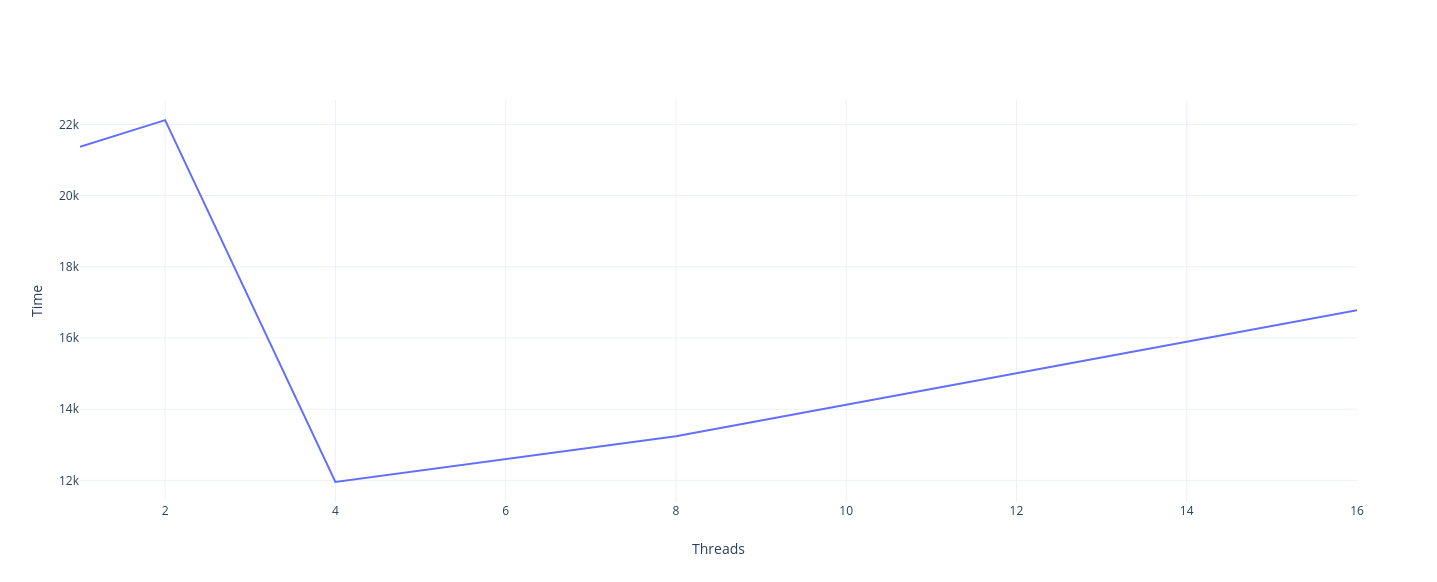
\includegraphics[scale=0.2]{graphic.png}
	\caption{Execution Time Graph}
\end{figure}


\end{document}
